\documentclass[11pt]{article}
\usepackage[T1]{fontenc}
\usepackage[utf8]{inputenc}
\usepackage{mathptmx}
\usepackage{microtype}
\usepackage{courier}
\usepackage[margin=1in]{geometry}
\usepackage{amsmath,amssymb}
\usepackage{graphicx}
\usepackage{booktabs}
\usepackage{tabularx}
\usepackage{caption}
\usepackage[numbers,sort&compress]{natbib}
\usepackage[hidelinks]{hyperref}
\usepackage{xurl}
\usepackage[section]{placeins}
\captionsetup{font=small,labelfont=bf}
\setlength{\parskip}{0.4em}
\newcolumntype{L}{>{\raggedright\arraybackslash}X}

\title{Who Beat Whom? A Weighted PageRank Ranking of Professional Tennis Players Compared with the ATP Ranking\\[0.4em]
\large Second draft}
\author{Chakib Madcur\\
\small Department of Computer Science, Roosevelt University, Chicago, IL}
\date{October 2026}

\begin{document}
\maketitle

\begin{abstract}
The official ATP ranking adds up points according to the tournaments a player enters and the rounds he reaches; it does not consider whom he beat. This paper studies an alternative based on network science. Each ATP season is represented as a directed graph in which every match is a directed edge from the loser to the winner, weighted by the number of wins over that opponent, and players are ranked with weighted PageRank (WPR). We compare WPR with the official ATP ranking using Spearman's rank correlation and cosine similarity, follow the comparison across the seasons 1973--2025, and contrast WPR with standard (unweighted) PageRank. We then apply the same method to football, American football, basketball, ice hockey and mixed martial arts, and place it within a classification of the approaches used to rank competitors in sports.
\end{abstract}

\noindent\textbf{Keywords:} weighted PageRank; directed graphs; network science; sports rankings; tennis.

%======================================================================
\section{Introduction}

The ATP ranking decides who enters tournaments, who is seeded, and who is called the best player in the world. It is a points system: a player receives fixed points for the round he reaches in each tournament, and the best results of the last 52 weeks are added up \citep{wiki_atp}. Two players who reach the same round of the same event receive the same points, whether they beat the world number one or a qualifier on the way.

Network science offers a different view. A season can be represented as a directed graph whose directed edges point from the loser of each match to the winner. In such a graph a strong player is one who beats other strong players, the idea behind PageRank \citep{brin1998}. In this paper the directed edges are weighted by the number of wins, and players are ranked with weighted PageRank (WPR).

The paper makes four contributions: (i) a comparison of WPR with the ATP ranking for every season from 1973 to 2025; (ii) a direct comparison of WPR with standard PageRank on the same directed graphs; (iii) an application of the same method to five other sports; and (iv) a first classification of approaches to ranking in sports.

%======================================================================
\section{Standard and weighted PageRank in sports}

Standard PageRank, designed to rank web pages, gives every directed edge the same weight \citep{brin1998}. The name \emph{weighted PageRank} was first used for web pages, where Xing and Ghorbani weighted each link by the popularity of the pages it connects \citep{xing2004}. In sports, the weight of a directed edge usually comes from the results themselves:

\begin{itemize}
  \item \textbf{Tennis.} Radicchi built a directed, weighted network of all professional matches from 1968 to 2010, in which the weight of a directed edge is the number of times one player lost to another, and ranked players with a PageRank-type ``prestige score'' \citep{radicchi2011}. Dingle et al.\ compared the same method with the ATP and WTA rankings \citep{dingle2013}.
  \item \textbf{American football.} Govan, Meyer and Albright weighted each directed edge by the score difference of the game and called this their first major generalization of PageRank \citep{govan2008}.
  \item \textbf{Football.} Lazova and Basnarkov weighted directed edges between national teams by combinations of wins and goals \citep{lazova2015}.
\end{itemize}

Weighting directed edges by the number of wins is therefore not new: it is how Radicchi's tennis network was built. Studies that use a network ranking usually choose one weighting and do not show what the weights change. Section~\ref{sec:std-vs-wpr} compares standard PageRank and WPR directly, across 53 seasons and several sports, and Section~\ref{sec:importance} tests a less common weight, the importance of the match.

%======================================================================
\section{Approaches to ranking in sports}

Table~\ref{tab:approaches} groups the methods used in sports into five approaches. Approaches 1 and 2 count results without looking at who the opponent was; approaches 3 and 4 take the opponent's strength into account; approach 5 has no direct opponent.

\begin{table}[!htbp]
\centering
\small
\caption{Five approaches to ranking in sports.}
\label{tab:approaches}
\begin{tabularx}{\textwidth}{@{}>{\raggedright\arraybackslash}p{3.1cm}LL@{}}
\toprule
Approach & Main idea & Examples \\
\midrule
1. League table & Points for each result over a season in which every team plays every other team & Premier League, NBA, NHL \\
2. Tournament points & Fixed points by event and round reached, added up over a time window & ATP and WTA rankings; UEFA club coefficients; ISU World Standings \\
3. Elo rating & A rating that moves after every match by the actual minus the expected result & FIDE chess ratings; FIFA Men's World Ranking since 2018 \\
4. Network rating & One calculation over the whole directed graph of results & Standard PageRank and WPR; Colley Matrix (college football) \\
5. Judged score & Judges score each performance; the highest total wins & Figure skating; gymnastics \\
\bottomrule
\end{tabularx}
\end{table}

\paragraph{1. League tables.} When every team plays every other team the same number of times, a points table is a fair ranking. English football adopted three points for a win in 1981, and FIFA adopted the system in 1995 \citep{wiki_3pts}.

\paragraph{2. Tournament points.} The ATP ranking belongs here. The first rankings, published on 23 August 1973, were based on each player's \emph{average} result. In 1990 they were replaced by a ``best of'' system that adds up a player's best 14 results; this became 18 results in 2000, and the last major overhaul of the points table was in 2009 \citep{wiki_atp}. Today a player's best 19 results count (plus the ATP Finals for qualified players), and points expire after 52 weeks \citep{wiki_atp}. During the COVID-19 pandemic the ranking was frozen on 16 March 2020 and then calculated from each player's best 18 results between March 2019 and December 2020 \citep{atp2020}; the usual method resumed on 23 August 2021, and all pandemic adjustments ended on 15 August 2022 \citep{tennismajors2021}. UEFA club coefficients add up points from European competitions over five seasons \citep{wiki_uefa}, and the ISU World Standings in figure skating add up points over three seasons \citep{wiki_isuws}.

\paragraph{3. Elo ratings.} Arpad Elo designed his system for chess \citep{elo1978}, and FIDE adopted it in 1970 \citep{wiki_elo}. After each match a rating changes by $K(S-E)$, where $S$ is the actual and $E$ the expected result, so a win over a stronger opponent earns more. FIFA has used an Elo-type method for its men's ranking since 16 August 2018 \citep{wiki_fifa}. In tennis, Elo is used by analysts rather than by the ATP \citep{fivethirtyeight2016,kovalchik2016}. The ATP ranking is \emph{not} an Elo rating: its points depend on the tournament and the round reached, not on the strength of the opponents beaten (the only exception is the United Cup, where points per win depend on the opponent's ranking \citep{wiki_atp}).

\paragraph{4. Network ratings.} These methods solve one problem over the whole directed graph of results: eigenvector methods \citep{keener1993}, direct and indirect wins \citep{park2005}, the Colley Matrix used in college football's Bowl Championship Series \citep{colley2002,wiki_colley}, and standard PageRank and WPR \citep{radicchi2011,govan2008,lazova2015}.

\paragraph{5. Judged scores.} In figure skating, competitors do not play each other. The ISU Judging System, used since 2004, scores each element as a base value plus a grade of execution and adds program component scores \citep{wiki_ijs}. Event results then feed the World Standings, so skating combines approaches 5 and 2.

\paragraph{Competition format.} Format matters as much as method. In a \emph{round-robin league} all teams face the same opponents. In \emph{knockout tournaments}, as in tennis, a player who loses leaves the event, so over a season each player meets a different set of opponents. Many sports use a \emph{league followed by playoffs}, and since 2024--25 the UEFA Champions League uses a \emph{league phase} in which each of 36 teams plays 8 different opponents \citep{wiki_ucl}. When schedules are incomplete, opponents differ from player to player, and approaches 3 and 4 have more to add \citep{zhou2020}.

%======================================================================
\section{Data}

\paragraph{Tennis.} We use Jeff Sackmann's ATP dataset \citep{sackmann}. For each season from 1973 to 2025 we take all tour-level main-draw matches (Grand Slams, Masters 1000, ATP 500 and 250 events, the ATP Finals, and the 2024 Olympic event) and remove Davis Cup ties, the Next Gen Finals exhibition and walkovers: 164{,}894 matches among 4{,}263 players. The 2025 season has 2{,}655 matches, 292 players and 2{,}395 directed edges. The official ranking is the last ATP ranking of each calendar year; its points are available from 1996.

\paragraph{Other sports.} Premier League 2025--26 (380 matches) \citep{footballdatasets}; NFL 2025 regular season (272 games) \citep{nflverse}; NBA 2025--26 regular season (1{,}230 games) \citep{hoopr}; NHL 2025--26 regular season (1{,}312 games) \citep{fastrhockey}, compared with the official points standings \citep{wiki_nhl2526}; and all decided UFC fights from 1994 to October 2026 (8{,}816 fights among 2{,}769 fighters) \citep{ufcdata}. We could not find an open, downloadable dataset of professional boxing results.

%======================================================================
\section{Methods}

\subsection{Directed graph}
For a season, each player is a node. Every match adds a directed edge from the loser to the winner; if the same player beats the same opponent again, the weight of that directed edge increases by one. Two players who beat each other are joined by two directed edges, one in each direction, each with its own number of wins (Figure~\ref{fig:h2h}). In leagues with draws or ties, a draw adds a directed edge of weight $0.5$ in each direction. Standard PageRank uses the same directed graph with every weight set to 1.

\begin{figure}[!htbp]
\centering
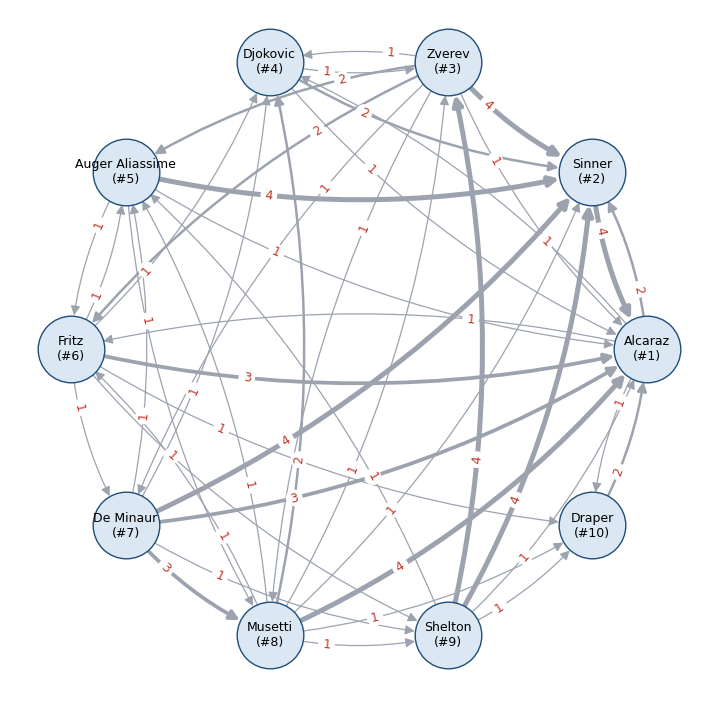
\includegraphics[width=0.6\textwidth]{figures/top10_head_to_head_2025.png}
\caption{Directed graph of the matches among the ATP top 10 of 2025. Each directed edge points to the winner and its label is the number of wins.}
\label{fig:h2h}
\end{figure}

\subsection{Weighted PageRank (WPR)}
WPR is the long-run behaviour of a random walk on the directed graph. A walker starts at a random player. At each step, with probability $d$ it follows one of the directed edges leaving the current player, that is, it moves from a loser to a player who beat him, choosing each directed edge with probability proportional to its weight. With probability $1-d$ it jumps to a player chosen uniformly at random; it also jumps uniformly when the current player has no losses. The WPR score of a player is the fraction of time the walker spends at that player. Players beaten by strong players are therefore visited often, and so are the players who beat them.

Let $w_{ji}$ be the weight of the directed edge from $j$ to $i$ (the number of times $i$ beat $j$), $s_j = \sum_i w_{ji}$ the total weight leaving $j$ (its losses), and $N$ the number of players. The WPR scores solve
\begin{equation}
\mathrm{WPR}(i) = \frac{1-d}{N} \;+\; d\sum_{j:\,w_{ji}>0} \mathrm{WPR}(j)\,\frac{w_{ji}}{s_j} \;+\; \frac{d}{N} \sum_{j:\,s_j=0} \mathrm{WPR}(j).
\end{equation}
We use $d = 0.85$, the value of the original PageRank \citep{brin1998}. All players have the same restart probability $1/N$; there are no node weights. We compute WPR by power iteration and check it against NetworkX \citep{hagberg2008} (largest difference $8\times10^{-12}$).

\subsection{Comparing two rankings}
Spearman's rank correlation $\rho$ \citep{spearman1904} is the measure most often used to compare two rankings, and it is our main measure. It compares the \emph{order} of the players. We also report cosine similarity \citep{manning2008}, which compares the \emph{scores}: for the ATP top $N$ we build the vector $\mathbf{a}$ of ATP points and the vector $\mathbf{p}$ of WPR scores and compute
\begin{equation}
\cos(\mathbf{a},\mathbf{p}) = \frac{\mathbf{a}\cdot\mathbf{p}}{\lVert\mathbf{a}\rVert\,\lVert\mathbf{p}\rVert}.
\end{equation}

\paragraph{Why cosine similarity and not Euclidean distance.} ATP points are in the thousands (12{,}050 for Alcaraz in 2025), while WPR scores are probabilities that sum to one (0.0489 for Alcaraz). The Euclidean distance between the raw vectors (about 20{,}000 for the top 10) mostly measures the size of the ATP numbers. Cosine similarity ignores the length of each vector and compares only the relations between players; it stays between 0 and 1 for positive vectors, so values for different $N$ can be compared. After both vectors are scaled to length one, Euclidean distance equals $\sqrt{2(1-\cos)}$ and carries the same information. Because all scores are positive, cosine is always positive, so we also report a random baseline: the mean cosine over 2{,}000 random permutations of $\mathbf{p}$.

\paragraph{Relation between the two measures.} With rank vectors $\mathbf{r}_a$, $\mathbf{r}_p$ and no ties,
\begin{equation}
\rho = 1 - \frac{6\sum_k (r_{a,k} - r_{p,k})^2}{n(n^2-1)} = \cos\big(\mathbf{r}_a - \bar r,\; \mathbf{r}_p - \bar r\big),
\end{equation}
so Spearman's $\rho$ is both a rescaled squared Euclidean distance between rank vectors and the cosine of the rank vectors after subtracting their mean.

%======================================================================
\section{Results}

\subsection{WPR and the ATP ranking in one season}
Table~\ref{tab:top10} shows the top 10 of 2025 by WPR. Eight of the ten are also in the ATP top 10, and the top two are the same. The largest differences are Alexander Bublik (4th by WPR, 11th by ATP) and Ji\v{r}\'i Leh\v{c}ka (9th and 18th). WPR also separates players with equal ATP points: in 2025, Brandon Nakashima and Stefanos Tsitsipas both finished with 1{,}380 points, and WPR places them 30th and 51st; in 2015, Ivo Karlovi\'c and Ga\"el Monfils both had 1{,}485 points, and WPR places Karlovi\'c 6th, because he beat Djokovic, Wawrinka and Berdych.

\begin{table}[!htbp]
\centering
\small
\caption{Top 10 by WPR, 2025 season, with the ATP year-end rank and the standard PageRank rank of the same players.}
\label{tab:top10}
\begin{tabular}{@{}rlrr@{}}
\toprule
WPR & Player & ATP rank & Standard PageRank rank \\
\midrule
1 & Carlos Alcaraz & 1 & 1 \\
2 & Jannik Sinner & 2 & 2 \\
3 & Taylor Fritz & 6 & 4 \\
4 & Alexander Bublik & 11 & 3 \\
5 & Novak Djokovic & 4 & 6 \\
6 & Alexander Zverev & 3 & 9 \\
7 & Felix Auger-Aliassime & 5 & 5 \\
8 & Alex de Minaur & 7 & 7 \\
9 & Ji\v{r}\'i Leh\v{c}ka & 18 & 10 \\
10 & Jack Draper & 10 & 12 \\
\bottomrule
\end{tabular}
\end{table}

\subsection{Standard PageRank and WPR}
\label{sec:std-vs-wpr}
Standard PageRank ignores how many times a player won. Consider four players: A beat B three times and lost to B once, A beat C three times and lost to C once, B and C beat each other once, and B also beat D. Standard PageRank sees one directed edge in each direction between A and B and between A and C, as if both head-to-heads were 1--1, and ranks B first (scores: B 0.336, A 0.313, C 0.313, D 0.038). WPR uses the 3--1 records and ranks A first (A 0.398, B 0.296, C 0.269, D 0.038).

The same thing happens with real data. In 2015 Djokovic went 81--6 at tour level, beat Wawrinka three times and lost to him once, and lost three of his six matches to Federer. Standard PageRank ranks Wawrinka first; WPR ranks Djokovic first, as the ATP did.

\begin{table}[!htbp]
\centering
\small
\caption{Agreement with the ATP ranking: standard PageRank and WPR.}
\label{tab:stdwpr}
\begin{tabular}{@{}llrrrr@{}}
\toprule
 & & \multicolumn{2}{c}{Spearman $\rho$} & \multicolumn{2}{c}{Cosine similarity} \\
\cmidrule(lr){3-4}\cmidrule(l){5-6}
Season & Players & Standard & WPR & Standard & WPR \\
\midrule
2015 & Top 10 & 0.879 & 0.952 & 0.928 & 0.978 \\
     & Top 50 & 0.807 & 0.849 & 0.880 & 0.966 \\
     & Top 100 & 0.928 & 0.936 & 0.877 & 0.964 \\
\addlinespace
2025 & Top 10 & 0.794 & 0.879 & 0.952 & 0.986 \\
     & Top 50 & 0.860 & 0.853 & 0.901 & 0.966 \\
     & Top 100 & 0.917 & 0.919 & 0.896 & 0.962 \\
\bottomrule
\end{tabular}
\end{table}

Across all seasons (Figure~\ref{fig:stdwpr}), WPR has a higher cosine similarity with the ATP points than standard PageRank in all 30 seasons from 1996 to 2025 (mean 0.963 against 0.925), and it picks the ATP's year-end number one in 24 of 53 seasons against 17. Spearman's $\rho$ is almost the same (mean 0.885 against 0.883, higher for WPR in 35 of 53 seasons): the weights matter most at the top of the ranking, where players meet each other repeatedly.

\begin{figure}[!htbp]
\centering
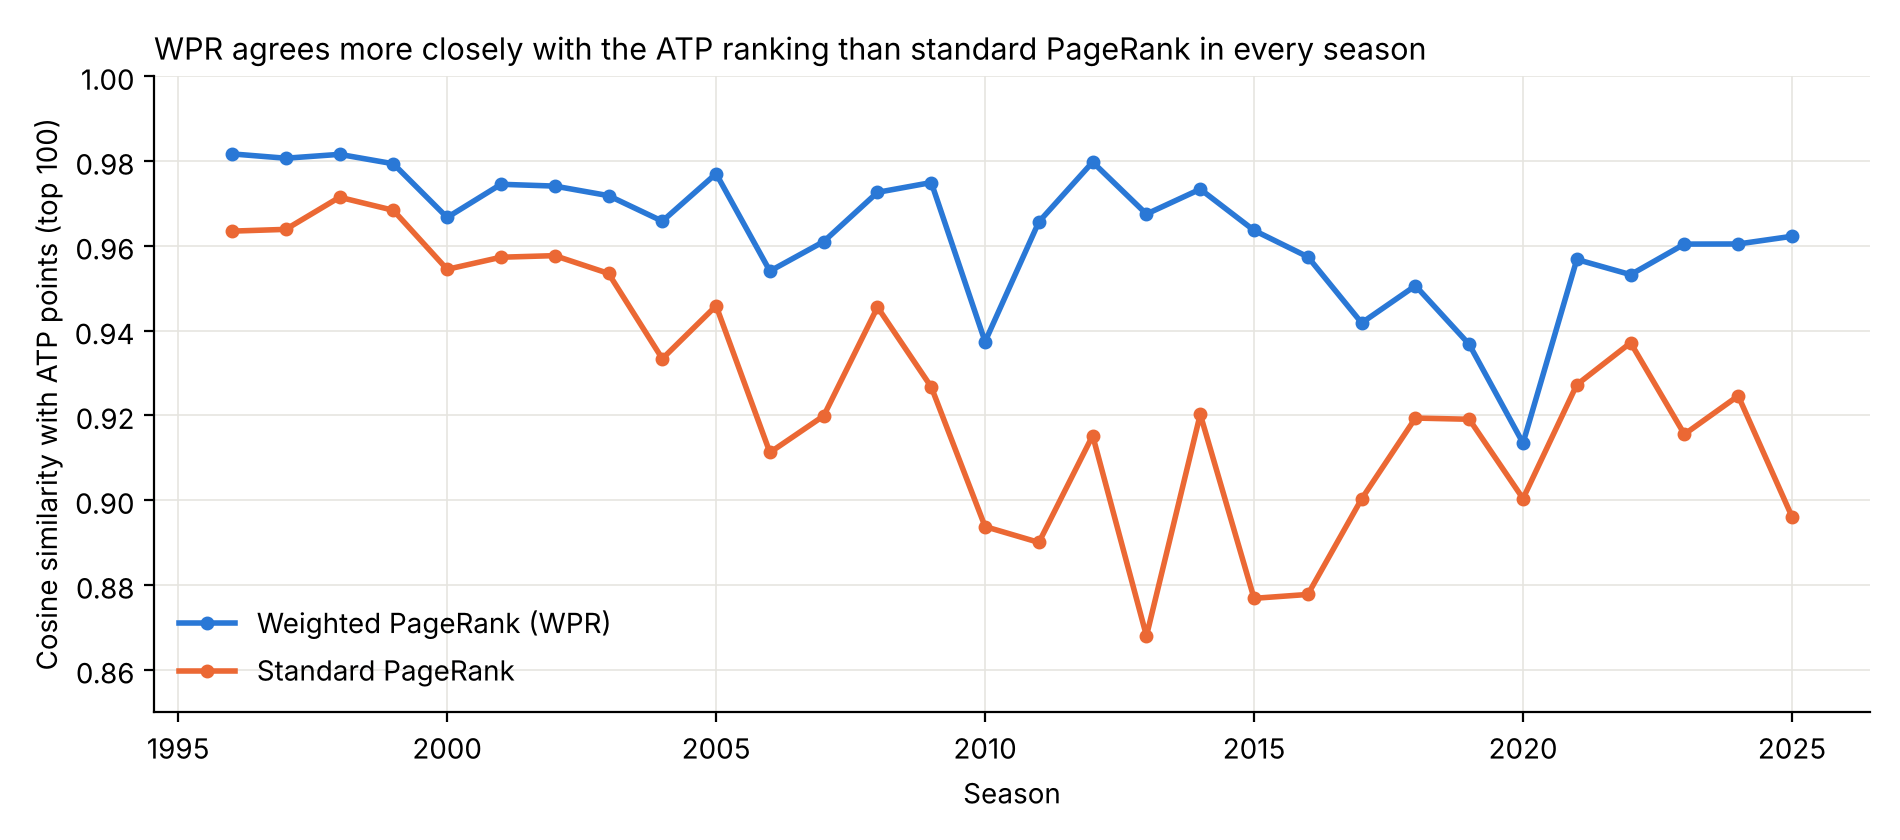
\includegraphics[width=0.85\textwidth]{figures/wpr_vs_standard.png}
\caption{Cosine similarity with ATP points (top 100) for WPR and standard PageRank, 1996--2025.}
\label{fig:stdwpr}
\end{figure}

\FloatBarrier
\subsection{Agreement for different numbers of players}
Table~\ref{tab:cosine} and Figure~\ref{fig:cosine} show cosine similarity between ATP points and WPR scores for the ATP top $N$. For $N \ge 10$ it is 0.96--0.99 in both seasons, while the random baseline falls from 0.73--0.78 at $N=10$ to 0.38--0.53 at $N=100$. With two players the comparison is not informative: the baseline is already 0.91 (2015) and 0.99 (2025). Table~\ref{tab:spearman} confirms the relation between Spearman's $\rho$ and cosine numerically.

\begin{table}[!htbp]
\centering
\small
\caption{Cosine similarity between ATP points and WPR scores for the ATP top $N$ (in 2015 one top-100 player played no tour-level match).}
\label{tab:cosine}
\begin{tabular}{@{}lrrrr@{}}
\toprule
 & \multicolumn{2}{c}{2015} & \multicolumn{2}{c}{2025} \\
\cmidrule(lr){2-3}\cmidrule(l){4-5}
Players & Cosine & Random baseline & Cosine & Random baseline \\
\midrule
Top 2 & 1.000 & 0.912 & 0.989 & 0.985 \\
Top 5 & 0.977 & 0.861 & 0.991 & 0.829 \\
Top 10 & 0.978 & 0.727 & 0.986 & 0.784 \\
Top 20 & 0.977 & 0.595 & 0.977 & 0.741 \\
Top 50 & 0.966 & 0.489 & 0.966 & 0.632 \\
Top 100 & 0.964 & 0.379 & 0.962 & 0.525 \\
\bottomrule
\end{tabular}
\end{table}

\begin{figure}[!htbp]
\centering
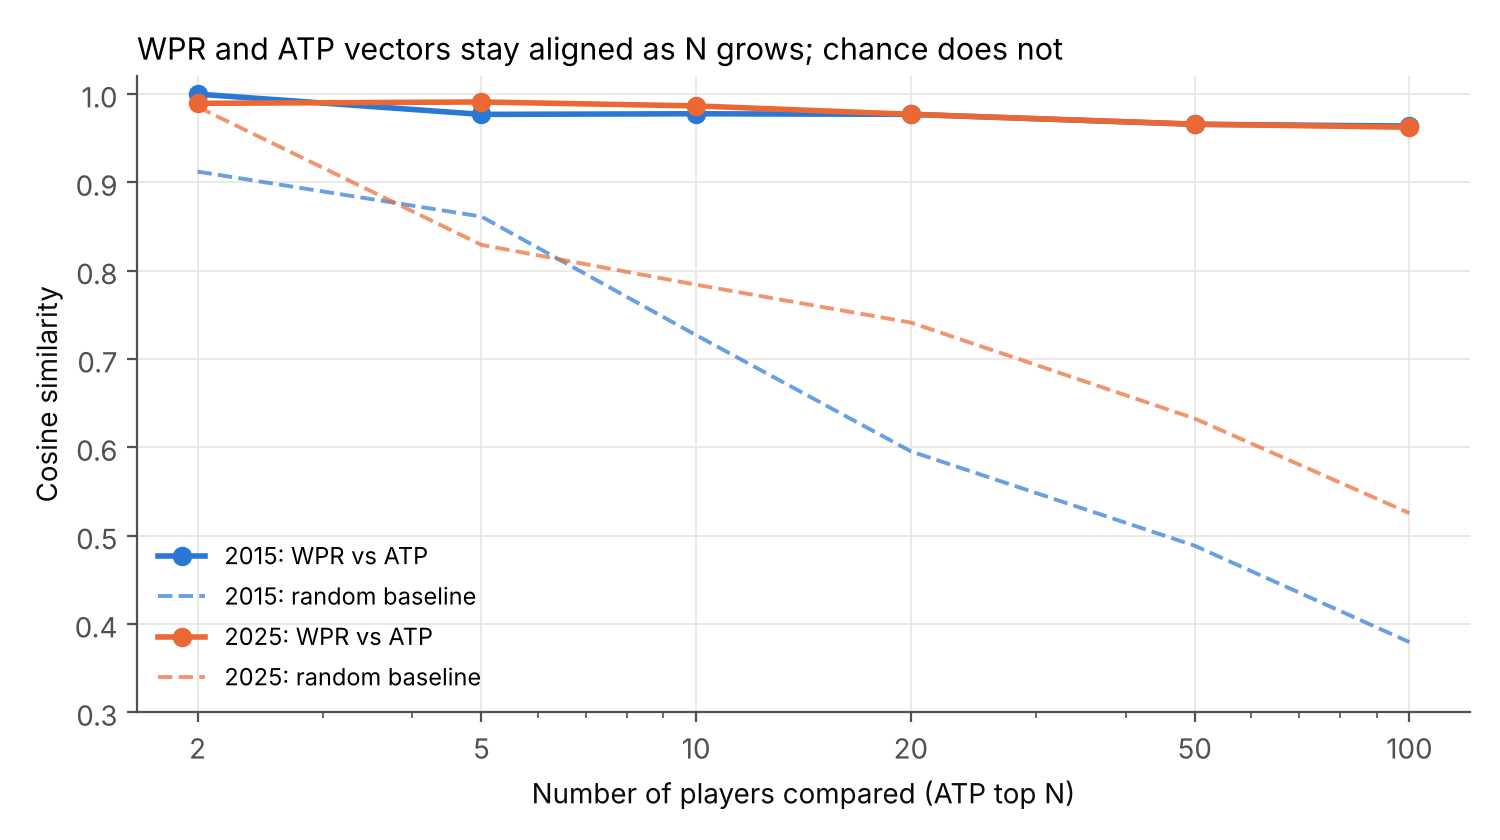
\includegraphics[width=0.75\textwidth]{figures/cosine_by_N.png}
\caption{Cosine similarity between ATP points and WPR scores (solid) and the random baseline (dashed).}
\label{fig:cosine}
\end{figure}

\begin{table}[!htbp]
\centering
\small
\caption{Three equal forms of Spearman's $\rho$, and cosine on scores, WPR against ATP, 2015.}
\label{tab:spearman}
\begin{tabular}{@{}lrrrr@{}}
\toprule
Players & Spearman $\rho$ & Centred cosine of ranks & $1-6\sum d^2/(n(n^2-1))$ & Cosine of scores \\
\midrule
Top 10 & 0.952 & 0.952 & 0.952 & 0.978 \\
Top 50 & 0.849 & 0.849 & 0.849 & 0.966 \\
Top 100 & 0.936 & 0.936 & 0.936 & 0.964 \\
\bottomrule
\end{tabular}
\end{table}

\FloatBarrier
\subsection{Agreement through time}
Figure~\ref{fig:time} repeats the comparison for the ATP top 100 in every season. Agreement was lower in 1973--1989, when the ATP ranked players by their average results (mean Spearman 0.848), than in 1990--2019 under the best-of system (0.910). The change coincides with the 1990 rule change, but 1990 is also when the ATP Tour began, so the data cannot separate the two. The clearest drop is 2020 (0.700): the year-end ranking covered March 2019 to December 2020, while the directed graph contains only the shortened 2020 season. Table~\ref{tab:seasons} lists selected seasons.

\begin{figure}[!htbp]
\centering
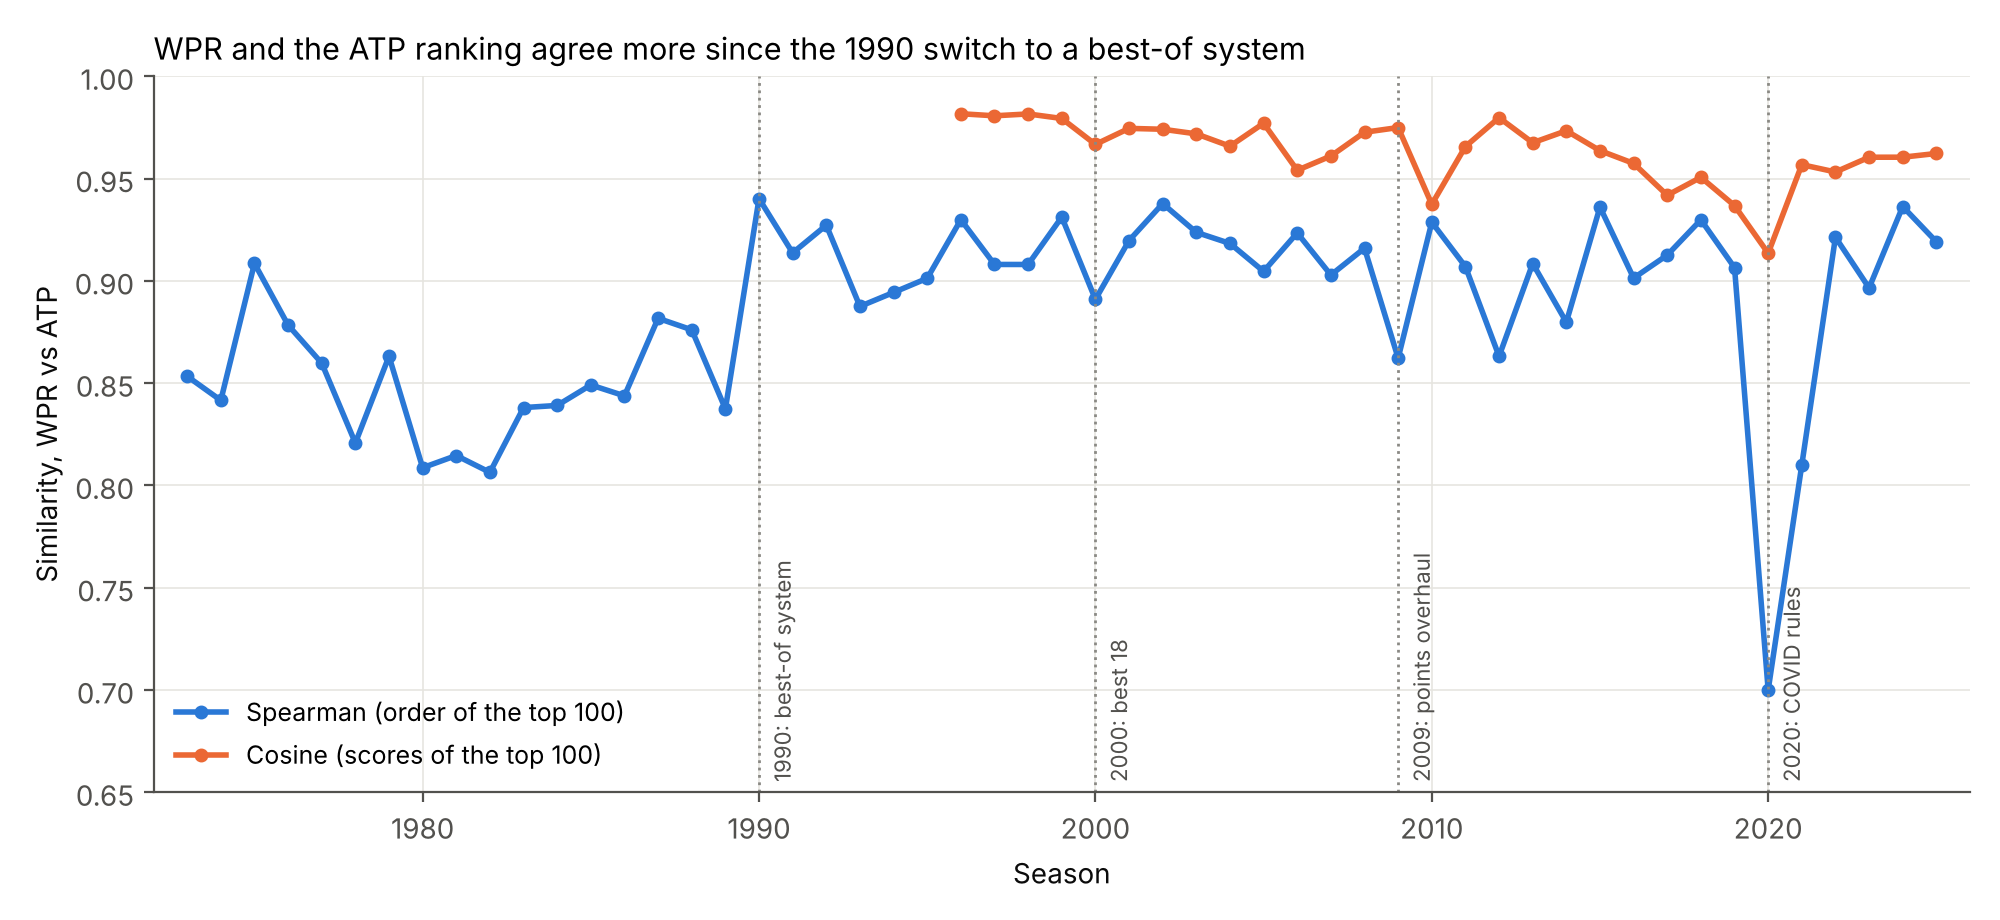
\includegraphics[width=\textwidth]{figures/agreement_through_time.png}
\caption{Agreement between WPR and the ATP year-end ranking (top 100) for every season. Dotted lines mark changes to the ATP ranking rules.}
\label{fig:time}
\end{figure}

\begin{table}[!htbp]
\centering
\small
\caption{Selected seasons: year-end number one in each system and agreement for the top 100.}
\label{tab:seasons}
\begin{tabular}{@{}rllrrr@{}}
\toprule
Season & ATP \#1 & WPR \#1 & Top-10 overlap & Spearman & Cosine \\
\midrule
1975 & Jimmy Connors & Arthur Ashe & 8 & 0.909 & -- \\
1978 & Jimmy Connors & Bj\"orn Borg & 7 & 0.821 & -- \\
1985 & Ivan Lendl & Ivan Lendl & 8 & 0.849 & -- \\
1990 & Stefan Edberg & Stefan Edberg & 8 & 0.940 & -- \\
1995 & Pete Sampras & Pete Sampras & 9 & 0.901 & -- \\
2005 & Roger Federer & Roger Federer & 7 & 0.905 & 0.977 \\
2010 & Rafael Nadal & Rafael Nadal & 8 & 0.929 & 0.937 \\
2015 & Novak Djokovic & Novak Djokovic & 8 & 0.936 & 0.964 \\
2020 & Novak Djokovic & Novak Djokovic & 8 & 0.700 & 0.913 \\
2022 & Carlos Alcaraz & Felix Auger-Aliassime & 9 & 0.921 & 0.953 \\
2025 & Carlos Alcaraz & Carlos Alcaraz & 8 & 0.919 & 0.962 \\
\bottomrule
\end{tabular}
\end{table}

\FloatBarrier
\subsection{Comparison with Elo}
Table~\ref{tab:elo} adds an Elo rating (tennis version with $K = 250/(m+5)^{0.4}$, run on all tour-level matches since 2005). WPR is closer to the ATP ranking than Elo, especially in 2025: Elo is built on a player's whole career and does not drop players who stop competing. Used to predict the winners of the first half of the next season, the year-end rankings perform almost equally (Table~\ref{tab:predict}).

\begin{table}[!htbp]
\centering
\small
\caption{Spearman's $\rho$ between each ranking and the ATP year-end ranking.}
\label{tab:elo}
\begin{tabular}{@{}llrrr@{}}
\toprule
Season & Comparison & Top 10 & Top 50 & Top 100 \\
\midrule
2015 & WPR vs ATP & 0.95 & 0.85 & 0.94 \\
     & Standard PageRank vs ATP & 0.88 & 0.81 & 0.93 \\
     & Elo vs ATP & 0.93 & 0.88 & 0.90 \\
\addlinespace
2025 & WPR vs ATP & 0.88 & 0.85 & 0.92 \\
     & Standard PageRank vs ATP & 0.79 & 0.86 & 0.92 \\
     & Elo vs ATP & 0.67 & 0.72 & 0.79 \\
\bottomrule
\end{tabular}
\end{table}

\begin{table}[!htbp]
\centering
\small
\caption{Share of matches in January--June of the next season whose winner each year-end ranking predicted (the higher-ranked player is predicted to win).}
\label{tab:predict}
\begin{tabular}{@{}lrrrrr@{}}
\toprule
Matches predicted & Number & ATP & Elo & WPR & Standard PageRank \\
\midrule
January--June 2016 & 1{,}509 & 67.1\% & 67.7\% & 66.8\% & 66.1\% \\
January--June 2026 & 1{,}202 & 63.7\% & 64.9\% & 63.1\% & 63.1\% \\
\bottomrule
\end{tabular}
\end{table}

\FloatBarrier
\subsection{Other sports}
Table~\ref{tab:leagues} applies WPR to four leagues. WPR is close to the final standings where every team plays every other team (NBA, Premier League, NHL). In the NFL, where teams meet only 45\% of the possible opponents, it differs more: it ranks the 12--5 Los Angeles Rams first and the 14--3 New England Patriots 11th, because the Patriots beat only one team with a winning record while the Rams beat five. In the Premier League, WPR ranks Manchester City first and champions Arsenal second, because City did better against the other top-six teams (5 wins, 2 draws, 3 losses against Arsenal's 3--2--5). In all four leagues standard PageRank is further from the standings than WPR, by 0.01 in the NFL and by up to 0.16 in the Premier League: where teams meet the same opponent several times, standard PageRank counts each pair only once.

\begin{table}[!htbp]
\centering
\small
\caption{WPR and standard PageRank against the final standings (Spearman $\rho$). ``Pairs met'' is the share of all possible pairs of teams that played each other.}
\label{tab:leagues}
\begin{tabular}{@{}lrrrrr@{}}
\toprule
League & Teams & Games per team & Pairs met & WPR & Standard \\
\midrule
Premier League 2025--26 & 20 & 38 & 100\% & 0.956 & 0.799 \\
NFL 2025 & 32 & 17 & 45\% & 0.888 & 0.880 \\
NBA 2025--26 & 30 & 82 & 100\% & 0.962 & 0.876 \\
NHL 2025--26 (official points) & 32 & 82 & 100\% & 0.875 & 0.815 \\
\bottomrule
\end{tabular}
\end{table}

UFC shows the limits of the method. Fighters meet only 0.22\% of the possible opponents, and many great fighters have a single loss. A fighter with one loss passes all of his score to the one opponent who beat him, so Matt Hamill (10--5) ranks 5th of all time because he holds Jon Jones' only UFC loss, a disqualification in 2009, and Adriano Martins (4--3) ranks 3rd because he holds Islam Makhachev's only UFC loss. In a very sparse directed graph, one upset can move a large share of the score \citep{zhou2020}.

\FloatBarrier
\subsection{Weights beyond win counts}
\label{sec:importance}
As a first step beyond win counts, we weighted each win by the importance of the match (Grand Slam 2, Masters 1000 and ATP Finals 1.5, other events 1). This raised the cosine similarity with ATP points in all 30 seasons from 1996 to 2025 (mean 0.975 against 0.963), while Spearman's $\rho$ hardly changed (0.904 against 0.901). The gain is partly expected, because ATP points also reward bigger tournaments.

%======================================================================
\section{Discussion}

\paragraph{Different approaches can give the same ranking.} WPR uses only who beat whom in one season; the ATP ranking uses a table of points by tournament and round. The two share no formula, yet their Spearman correlation for the top 100 lies between 0.80 and 0.94 in every season except 2020. Strong players both go deep in big tournaments and beat strong opponents, so both methods see the same signal.

\paragraph{Weights matter.} WPR agrees with the ATP ranking more closely than standard PageRank, and the difference is largest at the top of the ranking and in leagues where teams meet repeatedly. Counting each head-to-head only once can change who is first, as the 2015 Djokovic--Wawrinka example shows.

\paragraph{The disagreements are informative.} Where WPR and the ATP ranking differ, the reason is usually visible: players with equal points but different opponents, NFL teams with easy schedules, and years when the ATP rules changed (2020). Where WPR fails, as in the UFC, the reason is also visible: too few contests per competitor.

\paragraph{Limitations.} Each directed graph covers one calendar season, while the ATP ranking also counts Challenger results and only a player's best results. The damping factor and the importance weights are chosen, not learned. The other sports cover one season each. Several facts in Section~3 are taken from Wikipedia and should be replaced by official rulebooks.

%======================================================================
\section{Future work}

\begin{itemize}
  \item \textbf{When is WPR better than the ATP ranking?} Identify the situations in which each method gives the more sensible ranking, for example players returning from injury, players with few but strong wins, and surfaces.
  \item \textbf{Learned weights.} Learn the weights of the directed edges (tournament, round, surface, score, recency) from data instead of choosing them, including AI-based approaches.
  \item \textbf{Time.} Let older matches count less, so that the directed graph can span more than one season \citep{motegi2012}.
  \item \textbf{More sports.} Turn each figure-skating event into pairwise results between skaters, so that WPR can be applied to a sport without head-to-head matches, and find open data for boxing.
\end{itemize}

%======================================================================
\section{Conclusion}

Weighted PageRank built only from who beat whom gives rankings close to the official ATP ranking, closer than standard PageRank, and the cases where the two differ explain something real about the players. The same method nearly reproduces league tables in football, basketball and hockey, differs more in the NFL, where schedules are incomplete, and breaks down in the UFC, where competitors meet too few opponents.

\section*{Acknowledgments}
The author thanks Professor Evgeny Dantsin (Roosevelt University) for his guidance and feedback throughout this project.

\section*{Code and data availability}
All programs, notebooks and references are available at \url{https://github.com/ChakibMadcur/tennis-pagerank-research}.

\bibliographystyle{plainnat}
\bibliography{references}

\end{document}
